%% 
%% Copyright 2007-2020 Elsevier Ltd
%% 
%% This file is part of the 'Elsarticle Bundle'.
%% ---------------------------------------------
%% 
%% It may be distributed under the conditions of the LaTeX Project Public
%% License, either version 1.2 of this license or (at your option) any
%% later version.  The latest version of this license is in
%%    http://www.latex-project.org/lppl.txt
%% and version 1.2 or later is part of all distributions of LaTeX
%% version 1999/12/01 or later.
%% 
%% The list of all files belonging to the 'Elsarticle Bundle' is
%% given in the file `manifest.txt'.
%% 
%% Template article for Elsevier's document class `elsarticle'
%% with harvard style bibliographic references

%\documentclass[preprint,12pt,authoryear]{elsarticle}

%% Use the option review to obtain double line spacing
%% \documentclass[authoryear,preprint,review,12pt]{elsarticle}

%% Use the options 1p,twocolumn; 3p; 3p,twocolumn; 5p; or 5p,twocolumn
%% for a journal layout:
%% \documentclass[final,1p,times,authoryear]{elsarticle}
%% \documentclass[final,1p,times,twocolumn,authoryear]{elsarticle}
%% \documentclass[final,3p,times,authoryear]{elsarticle}
%% \documentclass[final,3p,times,twocolumn,authoryear]{elsarticle}
%% \documentclass[final,5p,times,authoryear]{elsarticle}
\documentclass[final,5p,times,twocolumn,authoryear]{elsarticle}
\usepackage{ctex}
\usepackage{url}
\usepackage{amsmath}
\usepackage{booktabs} % For professional looking tables
\usepackage{array} % For custom column alignment
\usepackage{graphicx}

%% For including figures, graphicx.sty has been loaded in
%% elsarticle.cls. If you prefer to use the old commands
%% please give \usepackage{epsfig}

%% The amssymb package provides various useful mathematical symbols
\usepackage{amssymb}
\usepackage{lipsum}
%% The amsthm package provides extended theorem environments
%% \usepackage{amsthm}

%% The lineno packages adds line numbers. Start line numbering with
%% \begin{linenumbers}, end it with \end{linenumbers}. Or switch it on
%% for the whole article with \linenumbers.
%% \usepackage{lineno}

%% You might want to define your own abbreviated commands for common used terms, e.g.:
\newcommand{\kms}{km\,s$^{-1}$}
\newcommand{\msun}{$M_\odot}

\journal{Teaching Assistant}


\begin{document}

\begin{frontmatter}

       \title{《金融数据分析与量化交易》实验报告}

       \author[first]{李甘 2023202296 信息学院}

       \begin{abstract}
              本次金融数据分析与量化交易实验中,
              我按照教程使用 tushare 下载了所有 2010 年以前上市的股票的日线数据,
              使用 PyTorch 深度学习框架训练了一个基于多层神经网络(MLP)的股票价格预测模型,
              并使用实验要求中提供的评测程序对自己的模型进行了评测。本报告中涉及到的全部代码、
              数据以及本报告的 \LaTeX 源代码已经上传至 GitHub 仓库:
              \url{https://github.com/Nictheboy/college-ids-hw/tree/main/lab}
       \end{abstract}

       \begin{keyword}
              %% keywords here, in the form: keyword \sep keyword, up to a maximum of 6 keywords
              量化交易 \sep 神经网络 \sep 深度学习 \sep MLP

              %% PACS codes here, in the form: \PACS code \sep code

              %% MSC codes here, in the form: \MSC code \sep code
              %% or \MSC[2008] code \sep code (2000 is the default)

       \end{keyword}


\end{frontmatter}

%\tableofcontents

%% \linenumbers

%% main text

\section{简述}
对金融数据的分析,尤其是对股票价格的直接预测,由于其直接的经济回报,一直是金融领域和机器学习领域的研究热点。
传统的分析方法有很多,比如基于技术指标的分析等,但是这些方法往往需要人工构造选取特征,模型很难自主从数据中学习特征。

与此同时,如何根据分析结果进行量化交易也是一个重要的问题。直接使用标注了交易信号的数据进行监督学习,
虽然可以得到在历史数据上表现良好的模型,但是在未来数据上的表现往往取决于标注的质量。
总的来说,基于技术指标和交易信号标注的方法虽然可以达到良好的效果,但训练过程中需要人工干预,难以挖掘数据中的潜在规律。

使用深度学习方法直接对股票价格进行预测,可以避免这些问题,因此在近年来受到了广泛的关注。
然而,由于股票价格数据本身的复杂性、过低的信噪比和博弈的性质,直接对股票价格进行预测是一个非常困难甚至本质上不可解的问题,
目前尚没有一个完全有效的解决方案。我作为一个普通的大二学生当然没有办法很好的解决这些问题,这些问题也因此构成了本次实验的主要困难。

由于我本人对金融了解甚微,我没有尝试对数据进行特征工程和交易信号标注,而是直接使用了数据中的股价信息训练预测模型。
同时,由于我对神经网络的了解也有限,所以我没有采用更为复杂的模型,而是使用了一个简单的多层神经网络(MLP)。本实验中,我借助
PyTorch 深度学习框架,训练了一个基于多层神经网络(MLP)的股票价格预测模型,尝试对股票下一日的价格进行预测,
并直接使用预测结果进行量化交易。

\section{环境搭建}
本实验使用 Python 3.13.1 作为编程环境。代码依赖\texttt{scikit-learn}、\texttt{torch}、\texttt{pyalgotrade}和\texttt{tushare}
四个包,可以使用 pip 安装:
\begin{verbatim}
pip install -r requirements.txt
\end{verbatim}

\section{模型训练}

\subsection{数据的获取}
深度学习往往需要海量的数据进行训练,因此本实验中,我并没有按照教程中的方法选取若干支股票进行训练,而是直接使用
tushare 平台下载了全部 2010 年以前上市的股票的日线数据(总计 1572 支股票),并使用教程中给出的代码对数据格式进行了转换。

用于下载数据的代码位于\texttt{download\_data.py},下载的数据保存在\texttt{data/download},
用于转换数据格式的代码位于\texttt{convert\_data.py},转换后的数据保存在\texttt{data/converted}。

\subsection{数据的预处理}
本模型只使用了数据中Open、High、Low、Close和Volume五列,因此预处理中我首先去除了其他列。

由于不同股票的价格差异较大,为了使模型更容易训练,我对数据进行了归一化处理。对实际交易最有价值的数据实际上不是价格本身,
而是价格的变化趋势,所以我采用的归一化方法是将每行都替换为该行数据与前一行数据的百分比变化。

用于数据预处理的代码位于\texttt{preprocess.py}。该文件提供了一个用于数据预处理的函数,该函数在训练模型和评测模型时都会用到。

\subsection{模型的搭建}
本实验中,我采用了一个多层神经网络(MLP)作为股票预测模型。该模型输入为前 33 天的股票数据(经过预处理,所以都是增幅数据),输出的期待值
\begin{equation}
       y = sigmoid(1 - e^{-20\alpha})
\end{equation}
其中\(\alpha\)为待遇侧的股价增幅。

该神经网络输入为5*33维,中间有6个2048维的层(激活函数为ReLU),最后通过sigmoid产生1维的输出。虽然这个神经网络结构简单,
但是由于其中间层庞大的规模,依然富有表达能力,可以学习到数据中复杂的规律。

为什么要这样设计输出的期待值呢?因为在交易中比多挣钱更为重要的是少亏钱,所以我希望模型在预测时对股价下跌的预测更为准确,
因此通过\(1 - e^{-20\alpha}\)对\(\alpha\)的正值进行压缩、负值进行放大,使得模型在预测时更加谨慎。
由于模型的sigmoid输出层只能输出0到1之间的值,所以我在构造预期输出时使用\(sigmoid(x)\)将输出值压缩到0到1之间。
采用这样的输出期待值,可以在一定程度上避免模型在预测时对股价上涨的预测过于乐观,在股价“跳水”前敏锐的察觉并抛售,从而在实际交易中减少亏损。

采用这样的输出期待值的另一原因是由于股价数据的信噪比过低,最初训练模型时,如果采用对陈的输出预期值,模型在训练中会收敛到输出一个固定的值0.5,
完全陷入局部最优,从而完全失去了预测的能力。通过这样的变换人为制造不对称性,可以在一定程度上避免这种情况发生,虽然我并不了解这其中的原理。
也许是因为神经网络本身一些数学上的性质,不对称的输出分布更不容易使得模型陷入“输出固定值”的局部最优,也有可能是因为一些金融上的原因,
预测股票的下跌比预测股票的上涨更为容易。总之实验表明,这种做法是有效的。

用于模型搭建的代码位于\texttt{model.py},用于构造训练数据集和测试数据集的代码位于\texttt{dataset.py}。

\subsection{模型的训练}
由于我的电脑显存有限,不能同时加载全部1572支股票的数据进行训练,因此我采用了分批次训练的方法。
考虑到每支股票的一些内在性质可能是不同的,为了避免某批次训练时过分的体现某几支股票的特点,我在每批次训练中都使用全部1572支股票的数据,
但每支股票都只选取10\%的数据。

在每批次的训练中,我选取了常用的BCE损失函数和Adam训练器,超参数选取为batch\_size = 512,epochs = 10,学习率手工从0.01逐渐降低至0.0001。
对输入的数据(即前面选取出的那10\%数据)进行1:9的测试集训练集分割,用于在模型训练中随时评价模型训练的效果。

为了避免发生训练中模型收敛到输出固定值的情况,我对模型输出的y值的统计学分布进行了监视。在y的标准差稳定到0.09后,
我在训练程序中加入了一旦y的标准差小于0.08就放弃本次训练的模型的算法。这有效避免了模型收敛到输出固定值的局部最优的情况的发生。

用于训练模型的代码位于\texttt{train.py},模型训练的日志位于\texttt{log/mlp-train.log},六列数据分别为每一个epoch训练结束后的时间、
在测试集上测得的Loss、以及在测试集上输出的y的平均值、标准差、最小值和最大值。

\section{模型的使用和评测}
由于\(y = sigmoid(1 - e^{-20\alpha})\)在股价增幅\(\alpha\)为正时大于0.5,在\(\alpha\)为负时小于0.5,
我简单地通过比较y和0.5来作出是否持有股票的决策。如果y大于0.5就持有,反之就不持有。如果昨天持有股票而今天模型认为不应该持有股票,就抛售,
反之就买入。

我对教程中提供的\texttt{MyTestStrategy.py}进行了最小幅度的修改以调用我的模型作出决策。

用于预测和决策的代码位于\texttt{predict.py},用于评测模型的实际交易效果的代码位于\texttt{judge.py},
该文件是修改教程提供的\texttt{MyTestStrategy.py}得到的。

评测程序每使用一支股票完成一次评测,就会向\texttt{log/judge/judge.csv}输出一行日志,该日志记录了评测时间、依据的股票数据的文件名、
模拟结束时的总剩余金额、总收益率、夏普指数、最大回撤和总交易次数。

\section{实验结果}
我对最终得到的模型进行了200次评测,并编写了\texttt{result\_statistic.py}对评测结果进行了统计,统计结果如表\ref*{tab:performance1} 所示。
表中的平均值和标准差统计时已除去离群值。由于这些股票数据的跨度多为10年左右,因此这里的回报率是10年的回报率。
可以看到,总的来说,本模型很好地进行了盈利。然而,虽然数据很漂亮,但实际上这里存在一个巨大的问题:
这里本质上是在测试集上运行测试。
\begin{table}[h!]
       \centering
       \begin{tabular}{@{}lcc@{}}
              \toprule
              \textbf{}             & \textbf{Avg ± Std}        \\ \midrule
              \textbf{Returns}      & $1239.82\% \pm 1039.76\%$ \\
              \textbf{Sharpe Ratio} & $0.75 \pm 0.26$           \\
              \textbf{Max Drawdown} & $41.40\%\pm 12.27\%$      \\
              \textbf{Trade Count}  & $601.32 \pm 57.92$        \\ \midrule
       \end{tabular}
       \caption{评测结果一}
       \label{tab:performance1}
\end{table}

为了纠正在训练集上测试的错误,我收集了新的数据并进行了测试。这些数据来自2010年到2011年之间上市的股票。
我们采用同样的方法对数据进行了处理得到表\ref*{tab:performance2} ,并发现,虽然收益率远不如在测试集上的表现,但依然是盈利的。
也就是说,这个模型在未知数据上也有一定的泛化能力。这一实验是成功的。
\begin{table}[h!]
       \centering
       \begin{tabular}{@{}lcc@{}}
              \toprule
              \textbf{}             & \textbf{Avg ± Std}      \\ \midrule
              \textbf{Returns}      & $159.38\% \pm 196.94\%$ \\
              \textbf{Sharpe Ratio} & $0.27 \pm 0.22$         \\
              \textbf{Max Drawdown} & $60.02\%\pm 13.24\%$    \\
              \textbf{Trade Count}  & $633.67 \pm 55.11$      \\ \midrule
       \end{tabular}
       \caption{评测结果二}
       \label{tab:performance2}
\end{table}

评测一的原始数据位于\texttt{log/judge/judge.csv},评测二的原始数据位于\texttt{log/judge/judge\_test.csv}。
同时,两次评测的各指标的分布图也分别于\ref{sec:performance1} 和\ref{sec:performance2} 给出。

\section{总结}
我使用了 PyTorch 深度学习框架训练了一个基于多层神经网络(MLP)的股票价格预测模型。
我对数据进行了预处理,构造了训练数据集和测试数据集,训练了一个简单的神经网络模型,并使用该模型模拟了量化交易。

我发现了一些有趣的现象,比如模型在训练时容易陷入局部最优,通过调整输出的期待值可以有效避免这种情况的发生。
虽然其中的具体原理我也只能作出初步猜测。

最后,我对模型的表现进行了评测,发现模型在测试集上表现良好。

\section*{致谢}
感谢覃雄派老师提供的宝贵教程!也感谢老师每周为我们提供的鼓励。当然,也不得不感谢ChatGPT为我提供的巨大的帮助。

毕竟,对一个可怜的不得不完成这一作业的大二同学而言,
没有教程的指导、老师的鼓励和工具的辅助,他怎么会能独立完成这样一个需要懂得很多量化交易和机器学习的知识才能完成的难题?

%% The Appendices part is started with the command \appendix;
%% appendix sections are then done as normal sections
\appendix
\newpage

\section{评测结果一}
\label{sec:performance1}
\begin{figure}[h!]
       \centering
       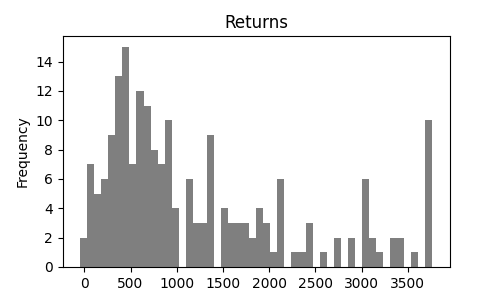
\includegraphics[width=0.37\textwidth]{img/1/Returns.png} % 指定图像文件名和宽度
       \caption{总回报的分布} % 添加图片标题
       % \label{fig:example} % 给图片添加标签用于引用
\end{figure}
\begin{figure}[h!]
       \centering
       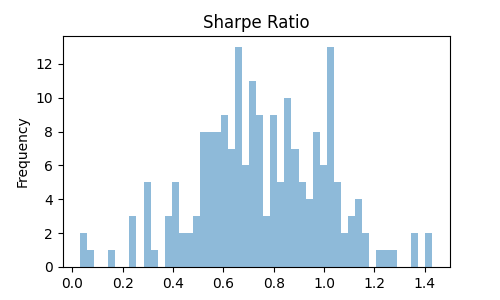
\includegraphics[width=0.37\textwidth]{img/1/Sharpe Ratio.png} % 指定图像文件名和宽度
       \caption{夏普系数的分布} % 添加图片标题
       % \label{fig:example} % 给图片添加标签用于引用
\end{figure}
\begin{figure}[h!]
       \centering
       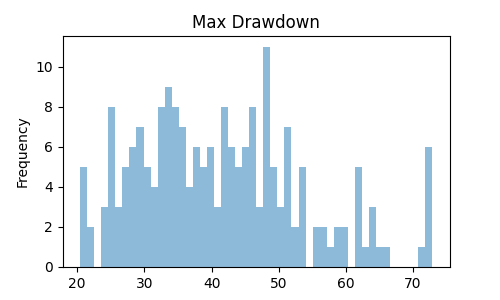
\includegraphics[width=0.37\textwidth]{img/1/Max Drawdown.png} % 指定图像文件名和宽度
       \caption{最大回撤的分布} % 添加图片标题
       % \label{fig:example} % 给图片添加标签用于引用
\end{figure}
\begin{figure}[h!]
       \centering
       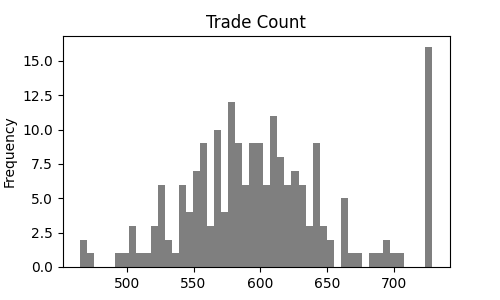
\includegraphics[width=0.37\textwidth]{img/1/Trade Count.png} % 指定图像文件名和宽度
       \caption{总交易次数的分布} % 添加图片标题
       % \label{fig:example} % 给图片添加标签用于引用
\end{figure}

\section{评测结果二}
\label{sec:performance2}
\begin{figure}[h!]
       \centering
       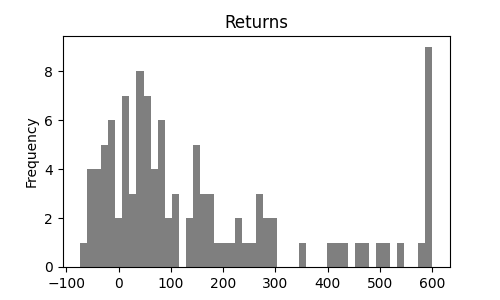
\includegraphics[width=0.37\textwidth]{img/2/Returns.png} % 指定图像文件名和宽度
       \caption{总回报的分布} % 添加图片标题
       % \label{fig:example} % 给图片添加标签用于引用
\end{figure}
\begin{figure}[h!]
       \centering
       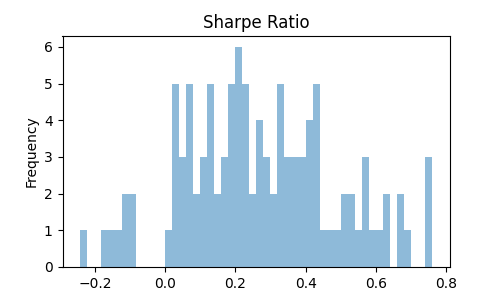
\includegraphics[width=0.37\textwidth]{img/2/Sharpe Ratio.png} % 指定图像文件名和宽度
       \caption{夏普系数的分布} % 添加图片标题
       % \label{fig:example} % 给图片添加标签用于引用
\end{figure}
\begin{figure}[h!]
       \centering
       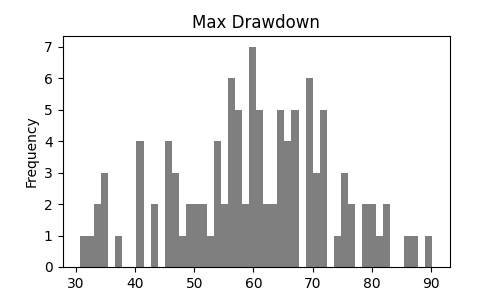
\includegraphics[width=0.37\textwidth]{img/2/Max Drawdown.png} % 指定图像文件名和宽度
       \caption{最大回撤的分布} % 添加图片标题
       % \label{fig:example} % 给图片添加标签用于引用
\end{figure}
\begin{figure}[h!]
       \centering
       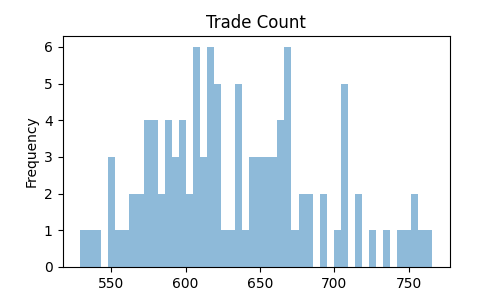
\includegraphics[width=0.37\textwidth]{img/2/Trade Count.png} % 指定图像文件名和宽度
       \caption{总交易次数的分布} % 添加图片标题
       % \label{fig:example} % 给图片添加标签用于引用
\end{figure}

%% If you have bibdatabase file and want bibtex to generate the
%% bibitems, please use
%%
\bibliographystyle{elsarticle-harv}
\bibliography{example}

%% else use the following coding to input the bibitems directly in the
%% TeX file.

%%\begin{thebibliography}{00}

%% \bibitem[Author(year)]{label}
%% For example:

%% \bibitem[Aladro et al.(2015)]{Aladro15} Aladro, R., Martín, S., Riquelme, D., et al. 2015, \aas, 579, A101


%%\end{thebibliography}

\end{document}

\endinput
%%
%% End of file `elsarticle-template-harv.tex'.

